\pdfoutput=1

\documentclass{l4proj}

\usepackage[english]{babel}
\usepackage{csquotes}
\usepackage{pdfpages}
\usepackage{float}

\begin{document}
\title{Deo: A Deontic Logic Theorem Prover}
\author{Leisha Hussien}
\date{2015/2016}
\maketitle

\begin{abstract}
Deontic logic, with its formalisation of concepts of obligation and prohibition, has many applications within Computer Science and beyond. This project proposes a formal specification and proof strategy for deontic theorems, with ethics applications as case studies. The final tool, Deo, comprises a grammar for semi-structured input and a brute force prover utility. It offers a user-friendly syntax and exhaustive proof strategy, including modus ponens, modus tollens and O-necessitation. It succeeds against implemented case studies, and provides thoughtful results for evaluation of ethics applications and deontic concepts, with scope for expansion over more complex case studies and various other areas of implementation. 
\end{abstract}

\educationalconsent

\tableofcontents

\chapter{Introduction}
\pagenumbering{arabic}

\section{Background and Motivation}
Deontic logic is a logic of duty, which is concerned with normative concepts of what should and should not be done. These concepts can include obligations, prohibitions and permissions, as well as the Hohfeldian incidents \cite{Hohfeld} of claims, powers, immunities and liberties. What is considered under the remit of deontic logic depends largely on what form of deontic logic is in use and the context it is being employed within. This project will largely be concerned with obligations, prohibitions and permissions, as they are the most relevant to the project under pursuit. While there is some disagreement about the proper meaning and correct definition of these concepts, for convenience, this project will employ largely conventional understandings. 

Concepts of obligation, prohibition and permission pervade everyday life, from legal proceedings to codes of ethics to database integrity. The exact content and use of these concepts varies from context to context, but understood abstractly and generally, they can provide a deeper understanding of these specific contexts and the problems faced within them. One area of particular interest is computational ethics, and what is necessary to create an ethical machine. One route is deontic, which would yield something like a Kantian machine \cite{Powers}. Showing that it is possible to operationalise the concepts in this way and get to some kind of automated reasoning would go some way towards showing that deontic computational ethics is at least possible. 

An interesting case study is codes of ethics, for example as part of university project proceedings. These vary depending on the kind of project being undertaken and the subject or subjects it is undertaken in, but broadly they can be understood as specifying the correct conduct of the researcher who will carry out the project, and sometimes the conduct of the body or bodies they will be reporting to over the course of it. This often includes, but is not limited to, the necessary procedures for dealing with human subjects, such as the provision of consent forms and the obligation to allow the removal of consent at any time. By very deliberately framing in deontic terms the content of the applications and the corresponding codes that must be adhered to, much of the extraneous detail can be removed, and the reasoning process required to determine acceptance of the application can be automated.

\section{Objectives and Achievements} 
This project aims to produce a deontic logic theorem prover, which will be henceforth referred to as Deo. This involves, first, the design and implementation of a formalisation of deontic logic, limited to the concepts of obligation, prohibition and permission. Within this formalisation, the atoms associated with a system, such as facts and rules, can be specified in a manner which allows for the automatic processing of these atoms. The specification of system in its processed form will be used by the prover, which will aim to show the success or failure of the desired goals of the system. 

Finally, the prover must be able to be tested against specific case studies, in order to determine the success of its implementation. The case studies used will draw on codes of ethics applications obtained from research projects submitted to the University of Glasgow for approval. Evaluation of the system will involve checking the results returned by the prover against the expected results and using the output to further assess the success of the implementation. 

The tasks carried out to achieve these objectives are as follows. First, various versions of deontic logic are identified and investigated in order to determine a specific version to be formalised. Next, a grammar to specify the expression of deontic statements is designed in order to produce a parser for the rules of a system. Then, from a file set out in this way, an abstract syntax tree is generated and stored. Finally, a prover is implemented that can be passed a specific logical axiom to then check whether this axiom coheres with the specified rules of the system.

The main objectives have been achieved. The finished product, Deo, comprises a formalised specification of deontic logic and a deontic theorem prover, which works as expected with the test cases and provides thoughtful results for evaluation. More complex testing and extension of the functionality is necessary to determine the true scope of the tool that has been produced, but it has gone some way towards showing that automating deontic reasoning about ethics is possible. 

\section{Structure}
This dissertation will first set out the history and development of deontic logic, including several of its various forms, as well as examining current and potential applications of deontic logic, before assessing any existing tool support for the issue presented. It will then explain the design and implementation of the implemented program, broken down into the lexical specification of the chosen form of deontic logic and the proof strategy for a given set of rules, facts and goals. It will then assess the system against several codes of ethics applications used as case studies. Once this is complete, conclusions will be presented about what the work done in the project shows, and potential avenues of future work will be suggested. 

\chapter{Literature Review}

\section{Development of Deontic Logic}
The development of deontic logic has been greatly influenced by alethic modal logic \cite{sep-logic-deontic}. Alethic modal logic is the logic of necessary truth, and its related operators are necessity, possibility, impossibility, non-necessity and contingency. Necessity is a basic operator; the other four operators can be defined in terms of it. What is necessary and contingent is possible, and what is contingent and impossible is non-necessary. Necessity maps loosely to obligation in deontic logic, as both can be thought of in terms of requirement. 

Deontic logic, as already explained, is a logic of duty. Duties can be understood in a Kantian sense, wherein the justification of maxims that are expected of agents is grounded in a respect for the laws which agents are bound to \cite{sep-kant-moral}. These laws can be anything from the moral law which can be said to govern all rational beings, to the legislation local to certain countries that applies only to their citizens, to the expected behaviour of an employee within a company under that company's code of ethics. In the chosen case study of this project, the maxims will be related to university codes of ethics, and more general expectations of good conduct from researchers. Relations between maxims, and how these should be formulated, will depend on the type of deontic logic in use. 

Deontic logic contains the usual operators of formal logic, such as negations, biconditionals, 
conjunctions and disjunctions. It can then incorporate many concepts, but here the focus will be on obligations, prohibitions and permissions. Obligations are those things which agents are required to do, prohibitions are those things which agents are forbidden from doing, and permissions are those things which agents are neither required to do nor forbidden from doing. As with alethic modal logic and necessity, obligation is a basic operator for deontic logic. The other operators of deontic logic can be constructed in terms of this basic operator. Prohibitions are things people are obliged not to do, while permissions are things people are neither obliged to do nor obliged not to do. 

Deontic logic says nothing about the content of deontic maxims, broadly speaking; where this is derived from is determined by deontological theories, which can be assessed for adequacy on their own terms. Indeed, in certain contexts, many deontological theories do not seem applicable for determing maxims, for example when these maxims concern database integrity. However, there is a clearer story to be told when dealing with codes of ethics. Following Kant \cite{groundwork}: 

\blockquote{It can lie nowhere else than in the principle of the will, regardless of the ends that can be effected by such action; for the will stands halfway between its a priori principle, which is formal, and its a posteriori incentive, which is material, as it were at a crossroads, and since it must after all be determined by something, it will have to be determined by the formal principle of willing as such when an action is done from duty, as every material principle has been taken away from it. The third proposition, as the conclusion from both previous ones, I would express as follows: duty is the necessity of an action from respect for the law. For the object as the effect of the action I have in mind I can indeed have inclination, but never respect, precisely because it is merely an effect and not activity of a will. Likewise, I cannot have respect for inclination as such, whether it is mine or that of another; I can at most in the first case approve of it, in the second at times love it myself, i.e. view it as favourable to my own advantage. Only what is connected with my will merely as ground, never as effect, what does not serve my inclination, but outweighs it, or at least excludes it entirely from calculations when we make a choice, hence the mere law by itself, can be an object of respect and thus a command.}

This is often described as the autonomy formula of the categorical imperative. Simply put, it states that the rational will should determine universal law. From this, an approach to validating sets of deontic maxims can be derived, which can thereby provide sets of laws. 

One convincing approach from machine ethics is ensuring that every maxim must be consistent with the rest of the set, and that the set must then form a coherent system of maxims \cite{Powers}. If there are inconsistent rules in the set, it is unreasonable to expect these maxims to be followed; it is impossible for $P$ and \( \neg \) $P$ to be true, so impossible for them to be justified coherently in a set. 

Powers derives two rules for this system: R-in and R-out. R-in states that a maxim, $m_i$ is allowed to be part of the set of acceptable maxims, $M$, if $m_i$ is consistent with the ethical system, $G$. That is, $m_i \in M \iff G \vdash m_i $. R-out states that if a maxim, $m_i$, becomes inconsistent with the ethical system, $G$, $m_i$ is no longer allowed in the set of acceptable maxims, $M$. That is, $m_i \notin M \rightarrow \neg(G \vdash m_i)$. These rules would be difficult to operationalise, but a successful implementation would provide useful analysis of sets of rules formulated in a deontic way. 

\section{Types of Deontic Logic}

\subsection{Standard Deontic Logic}
Standard deontic logic is a monadic logic which extends propositional logic. If $O$ represents obligation, the concepts can be formalised as follows: if $A$ is some obligation, then $O(A)$; if $A$ is some prohibition, then $O$(\( \neg \)$A)$; if $A$ is some permission, then \( \neg \)$O(A)$ \& \( \neg \)$O$(\( \neg \)$A)$. For example, if there is a prohibition on murder, and the action of murder is represented by $A$, this can be represented as $O$(\( \neg \)$A)$. Nothing more needs to be done to show that $O(A)$ holds once $A$ is proven to be true. 

Standard deontic logic faces the contrary-to-duties problem. It is not implausible that it could be forbidden that $C$, but in the case of $C$, it could still be expected that $A$. The classic example is of the gentle murderer; murder is forbidden, but if an agent is going to commit murder, they are obliged to do it in a way that causes the least amount of suffering. Standard deontic logic could represent these cases as follows: a general prohibition on murder and the action of murder is represented by C. If an agent is committing murder (C) they are obliged to murder gently (A). This contrary-to-duty obligation can be represented by $O(A)$. Taken together, these two obligations can be represented as $O$(\( \neg \)$C)$ \& $C$ \( \to \) $O(A)$. However, there is no way that $C$ and \( \neg \)$C$ can both be true; if C is true, it necessitates the falsehood of $\neg C$. 

\subsection{Non-Monotonic Deontic Logic}
Non-monotonic deontic logic introduces consistency \cite{Powers}. This is useful both for dealing with the kind of conflicting obligations detailed above and for handling conditional obligations \cite{Horty}. Following Reiter's symbolisation of default logic \cite{Reiter}, if $A$ is an obligation, and $C$ is some condition that $A$ must be consistent with in order to hold, \( \frac{C : O(A)}{O(A)} \). This also neatly handles the contrary-to-duties problem; if there is a general prohibition on murder, and the action of murder is represented by C, but if in the context where an agent is committing murder they are obliged to kill gently and this can be represented by O(A), then \( \frac{C : O(A)}{O(A)} \). The justification is the same as the conclusion, and is true only in the case of there being no facts, or defeater conditions, which would make it false. 

Dyadic deontic logic is a non-monotonic logic which introduces a context as a way to respond to the contrary-to-duties problem. Rather than there being simply an ideal world, where duties are fulfilled, and a non-ideal world, where they are not, there can be more or less ideal worlds depending on the number of obligations that are fulfilled. In dyadic deontic logic, if $A$ is an obligation that only applies given a context $C$, $O(A$ \textbar $C)$ and so following. This allows for seemingly contradictory statements such as $O($\( \neg \)$C)$ \& $O(A$ \textbar $C)$ to coexist without conflict. For example, if there is a general prohibition on murder, and the action of murder is represented by $C$, but if in the context where an agent is committing murder they are obliged to kill gently and this can be represented by $O(A)$, then $O($\( \neg \)$C)$ \& $O(A$ \textbar $C)$. 

However, despite effectively capturing an important aspect of reasoning, non-monotonic logic fails a first-order logic requirement for semi-decidability of set membership. It cannot guarantee whether a maxim is forbidden or obliged, even when it is in fact one of the two, which is problematic for a formalised system. 

\subsection{Predicate Deontic Logic}
Predicate logic introduces quantifiers, which allow for specification of what statements actually refer to. Statements can range over all members of a group, (at least) one member of a group, no members of a group or not all members of a group. If $x$ is some agent and $A$ is some obligation incumbent upon all of $x$, \( \forall{x(O(A))} \). 

For example, the general prohibition on murder, ($A$), which applies to all rational beings, ($x$), can be represented as \( \forall{x(O( \neg A))} \). To show the distinction, if all citizens ($x$) are obliged not to murder, but officers of the law ($y$) are permitted to murder in certain cases, this can be represented as \( \forall{x(O( \neg A))} \) \& \( \forall{y( \neg O( \neg A) \& \neg O(A)} \). These are not contradictory maxims in predicate logic, so it allows for much more complex sets of deontic rules. 

A further benefit of predicate deontic logic is that it does not face the traditional problems levelled at deontic logic \cite{predicate}. However, since it brings in concepts from logic of action, it is outside of the scope of this project and will not be explored here. 

\section{Applications of Deontic Logic}
Deontic logic lends itself well to applications within law, due to the aforementioned grounding in a respect for laws. One way to implement this is to characterise the law as a system of norms, as Jones and Sergot suggest \cite{law-jonessergot}, before going on to represent this system of norms using deontic expressions. They propose an important test to employ when assessing whether a deontic formulation of a state of affairs is appropriate. Firstly, there must be a sense in which it is possible that a prescription can be violated. Secondly, this violation must lead to a new state of affairs which needs an explicit representation in order to achieve the goals of the system. 

Applications within Computer Science have largely grown out of legal applications. Wieringa and Meyer categorise these as follows \cite{meyer93applications}: fault-tolerant computer systems, normative user behaviour, normative organisation behaviour and normative behaviour of the object system. Most of these applications use deontic logic to model some form of ideal behaviour, and what should be done in the case on non-ideal behaviour. Fault-tolerant computer systems can apply deontic concepts as a kind of exception handling process, by specifying what should happen when constraints on the expected behaviour of the system are violated. User behaviour is frequently non-ideal; ideal and actual user behaviour can be distinguished, simplifying the specification of such, and so normative user behaviour can also be considered an application of deontic logic in terms of exception handling. 

Wieringa and Meyer split applications within organisations into policy specification and normative organisation behaviour. This behaviour is a similar application to the legal domain, as organisations are required to follow the law. Within policy specification, deontic concepts can be used to specify the behaviour of various components of an organisation, removing ambiguity from organisational policies and making clearer the consequences of violations of policy. As with normative organisation behaviour, policy specification is similar to legal applications in terms of its implementation; the only difference is that these policies are not legally binding. While deontic logic cannot be used within secure computer systems as these systems do not allow for the violation of security norms, it can be used to formalise security policies for the exploration of the consequences of such policies, as well as for a potential proof that the policy is actually implemented by a certain system. 

One application within policy specification is system availability \cite{brunel04deontic}. After extending the logic with temporal operators, so it can be said that some obligation, $A$, needs to be done before a certain time, $k$, this obligation can be formally represented. From this, simple availability policies can be defined, and then checked for consistency. Violation of these policies is also easy to verify, as it can be checked whether the system is in accordance with all of the defined rules. 

Finally, deontic logic can be applied to normative behaviour of the object system, which is some part of reality whose data can be represented. Wieringa and Meyer split this application further into the specification of law, simulating legal thinking, specifying integrity constraints and any other possible application outside of these. Within the specification of law, there are vast opportunities for deontic logic to be employed. A formalised system can be used either as a tool for students to learn about law, or as a kind of oracle for the legislative process or for the application of legislation, or even to issue authoritative commands. The simulation of legal thinking moves away from the formal specification of actual laws towards how the law is actually thought about by those who are to implement it. Instead of using deontic logic to constrain the behaviour of the system, it can be used to describe the kinds of behaviour that actually occur in the system. Specifying integrity constraints is a similar application to the specification of law, in terms of implementation; only the context in which the implementation occurs is different. In terms of other possible applications, one mentioned is scheduling problems. Deontic logic can be used to specify the allocation of resources within certain constraints, and what should happen in the case of a violation of a constraint. 

A further application in this area is the specification of information systems \cite{infosystems}, particularly with respect to soft constraints. Dyadic deontic logic, with its ideal and non-ideal worlds, can neatly describe what is going on when there is some constraint of a system that ideally should not be violated, and what should be done if it is. 

An additional application to those mentioned above is responsibility modelling \cite{responsibility}. Responsibility, for an agent, can be defined in three different ways. Firstly, an agent can be considered responsible if something bad happened that the agent could have prevented. Within Computer Science, this is often manifest in a concern for security requirements, and analysis of their failure. Secondly, an agent can be considered responsible if they are obliged to report their actions to some authority figure. This definition is particularly useful for the consideration of policies which regulate interaction between users and information systems. Finally, an agent can be considered responsible if they are accountable for their actions and must be able to justify them. This definition can enable analysis of an agents' actual capabilities with their defined responsibilities. Both the second and third definition are both easily formulated in deontic terms of obligation and prohibition. This formulation can provide useful models of systems for understanding responsibility, and for the analysis of requirements and regulations. 

Wieringa and Meyer raise several issues with the application of deontic logic in the manners discussed above, namely the issues of possibility and authority. Computer Science frequently borrows concepts from other disciplines, only to recreate simplified versions of these concepts for its own purposes. With respect to the law, the version that appears in formalised specifications is frequently quite simplistic, and often reduces it to the application of rules to facts, as this is the way in which a computer can process something as complex as the law. It is important to consider the way in which humans practice and apply normative concepts differs to a computer's methodology. Both must interpret the available facts and apply rules within the area of the law in order to make a decision, but humans are able to provide more nuanced interpretations of a situation, while computers are bound by the given facts and rules. It may be tempting to think of this as a benefit, with computers forced to be impartial towards particular cases, but it is important not to lose sight of such things as programmer biases, which are inherent to the programs they create. This raises concerns as to the possibility of a genuine formalised system which can apply deontic concepts in anything like a satisfying manner. 

However, Wieringa and Meyer propose a set of conditions, which, should they be met, at least give conditions for the application of deontic logic within Computer Science to be practically feasible. These are as follows: the area of the law chosen for formalisation must be largely isolated from other areas of law, so as to keep the system at a manageable size; the application of the chosen area must not be very complicated, and must be largely basic common sense, since the representation of common sense reasoning in computer systems is deeply difficult; and the chosen area must not be subject to change, in order to avoid the incorporation of social learning into the system, as well as to avoid having to continually change the formalisation of the law. 

A further problem with these kinds of applications is the issue of authority. If a deontic system is used to issue authoritative commands, a possibility suggested above, then it is important that the system has to authority to do so, or its commands will have no actual effective force. It is definitely possible for a computer system to have such an authorative force, but it will not be immediately obvious from its existence alone, as it is with a human authority figure. While human authority figures are also subject to legal obligations, prohibitions and permissions, computer systems do not bear responsibilities in this way. In order for its authority to be respected, the fact that it has authority must be made clear to all participants of the system, a feat which is hardly easy to achieve. 

\section{Existing Functionality}
In the area of research applications and codes of ethics, one existing tool is the NHS Health Research Authority Decision Tool \cite{NHS}. This includes a set of toolkits and linked decision tools. The set of toolkits includes a clinical trials toolkit, which guides the user through the requirements for testing medicine; a data and tissues toolkit, which guides the user through  the requirements for using human data or human tissue in research; an experimental medicine toolkit, which guides the user through the requirements for interventional research; and a UK stem cell toolkit, which guides the user through the requirements for the research and manufacture of stem cells. The decision tools allow the user to check whether some project the user is pursuing should be categorised as research, or whether the project will require approval from an NHS research ethics committee. The focus of the set of toolkits is largely on making the user aware of their obligations as a health researcher, which is relevant to the concerns of the project, but less relevant to the end goal of a theorem prover. 

More relevant to the overall project is the decision tools, which follow some kind of verification process, given some facts from the user, to make a decision for the user as to either the status of their project as research, or whether their project will require approval. It is not, however, implemented in a deontic way, even if its aims can be framed and understood as such, so its considerations will be slightly different from the considerations of this project. 

\subsection{KED}
There has been relatively little work done in the area of deontic theorem proving. One tool which has been explicitly developed to operationalise deontic logic is KED \cite{KED}, a deontic theorem prover implemented in Prolog. It builds on work done to create KEM \cite{KEM}, which is a modal theorem prover implemented in Prolog. It works with standard deontic logic, making use of modal logic and its possible worlds semantics \cite{sep-possible-worlds}. The prover itself works by constructing a proof by contradiction, by first assuming that the formula to be proven is false and then exploring all the possible alternatives in an attempt to find formulae which contradict this assumption, closing off every created branch until it can be shown that the formula to be proven is, in fact, true. The proof strategy consists of $\alpha$ rules, which borrow the tableau method of proof's linear branch-expansion rules, as well as $\beta$ rules, which are rules of inference such as modus ponens and modus tollens. Together, these rules should provide a complete prover for this context. 

Importantly, KED is based on Mondadori's classical proof system \cite{Mondadori}, which itself is based on the tableau method but is much more concise and efficient. KED's proof strategy avoids the traditional redundancy involved with the tableau method by restricting the use of rules to only unfulfilled subformulae in the current branch, thereby limiting the size of the search space. Two key theorems for KED are proposed. The first is that a canonical KED tree always terminates, because of the fact that at every step of the process, there are a finite number of new, less complex formulae created, and as well as the fact that the number of possible labels in the tree for a formula to be proven is limited by the number of modal operators of the formula. The second theorem is that a KED tree for a formula to be proven is closed if and only if the canonical KED tree for that formula is closed, because a KED tree explores all the possible alternatives that can lead to closure of the constructed tableau. A further benefit is that there is no preprocessing of input formulae required. KED works using labels, so it lends itself to more natural proofs with simple implementations. While its implementation was limited to standard deontic logic, the implementation is flexible and generic enough that it can easily be extended to cover more, non-classical logical systems, such as multi-modal logic. 

\subsection{ESPLEX}
A further tool is ESPLEX, which, while not explicitly a deontic theorem prover, formalises legislation in a deontic way in the field of agricultural tenancies \cite{ESPLEX}. It aims to calculate the normative consequences of a case by providing possible configurations of the various deontic prescriptions. Like KED, it is implemented in Prolog, and aims to reproduce the language of legislative texts as closely as possible. The formalised language is required to be rich enough to convey the various levels of meaning within the texts, well defined on both a syntactic and semantic level, diverse enough to represent various different characteristics and aims, and flexible in its ability to allow the knowledge base to be continually updated. As a logical programming language, Prolog is well suited to meet these aims; its proof strategy is very similar to the activities involved with the manual processing of legislation. However, it is important to note that ESPLEX does not deal with the problem of negation as failure; this is dealt with at the meta level, by making a distinction between the two types of negation. 

A key distinction is made between explicit and implicit knowledge, and how these two different kinds of knowledge are formalised within the tool. Explicit knowledge is represented through logical rules, while implicit knowledge is represented within the semantic network. The logical rules can represent five different types of sentence: goal, which is a statement of what is obligatory, forbidden or permitted; fact, which is a statement of some fact of the system; cond, which is a statement of some condition of the system; def, which defines some legal status; and proc, which defines some legal procedure. As for the semantic network, these are binary relations on elements of the knowledge. These relations are `is a', `part of', `attribute', `value', `event', and `equal to'. 

ESPLEX's knowledge base can be accessed in a number of ways. Firstly, the rule set can be searched by selecting some goals, along with a calculation of the normative consequences of these goals. It can then provide the justification for its reasoning, or examine a normalised version of the steps followed to reach this justification, or evaluate the consequences in deontic terms, or analyse the action, parties or objects involved in the search for a solution. Secondly, the system can search the network for a desired entity by either identifying the entity to the user, visualising the properties of the entity, or determining the values of the properties of the entity. The final result is an outline which consists of both definitional and normative content, and is organised according to the jurisprudence on the elements of the case. Thirdly, the system can analyse characteristics of a legislative text. It can then visualise the definitions contained therein, and compare the procedural rules applied as well as the prescribed actions, evaluating these in deontic terms. 

While ESPLEX's existing functionality is incredibly useful, there are multiple possible extensions of the system. One point of particular interest is the ability to verify the normative coherence and completeness of a piece of legislation, as has been previously highlighted in this review \cite{Powers}. 

\subsection{TAXMAN}
TAXMAN models concepts within the legal area that applies to corporate reorganisation \cite{TAXMAN}, and is implemented primarily in Micro-PLANNER, which is a subset of PLANNER. It stores the facts of such a reorganisation and uses formalised definitions of the legislation to determine whether or not it can be considered a tax-free transaction. It considers some classical problems in legal reasoning with regards to legal concepts, such as their structure, the process by which they are transformed and modified, and the arguments usually made with respect to them. TAXMAN's own reasoning is fairly simple; it is able to analyse the facts of a corporate reorganisation case in terms of legal concepts. As with ESPLEX, TAXMAN considers it important for the area of law it is concerned with to be sufficiently complex, but also simple enough that a model of the system can be generated in a reasonable amount of time. 

An important first step for TAXMAN is completing the task of semantic information processing. In order to model corporate reorganisations, it needs to be able to express fundamental propositions about corporations, as well as more abstract concepts regarding reorganisation law, such as stock distribution. It must maintain a model of the corporate world in its knowledge base, which contains such entities as corporations and stocks. It also needs some fundamental operations that it must perform in order to manipulate this model of the world. This includes storing a list in its memory, retrieving a list from its memory, and deleting a list from its memory when necessary. Storage and deletion is done using, respectively, the commands ASSERT, which stores and indexes a list for future retrieval and makes it true in the world of the model, and ERASE, which removes the list from memory and makes it false in the world of the model. For memory retrieval, the GOAL command is used, which uses pattern matching for its search process. Importantly, the procedures defined in TAXMAN's system are as flexible as a programming language, so they are much more powerful than they would be as defined within symbolic logic. It has all the benefits of a programming language, such as dealing appropriately with updates to the knowledge base, as well as being able to deal with a structured, complex environment, and deal with it efficiently. 

One case study implemented in TAXMAN is United States v. Phellis, some of the facts of which could not be represented in the system as it stands. The case study is important in showing that it is possible to match reorganisation patterns to the network of a case description. It highlights multiple matches, including partial matches, which shows there are many ways to manipulate the concepts of corporate reorganisation law, as well as illuminating the potential for ambiguity in analysis of this area of law. This is a key benefit of the system, and it could be extremely powerful if it could overcome its limitations. TAXMAN, as it stands, does not have a particularly extensive coverage within law, and were it to be extended, the nature of the input required to the system means it is not very accessible to the users who would be most likely to use it. 

\section{Conclusions}
This review yielded some important considerations for the project. Firstly, the form of deontic logic implemented will be standard deontic logic. This is because it lends itself well to formalisation, as well as being easily extendable to other forms of logic if this is desired in future work. From the review, it is clear that flexibility and extensibility are important non-functional requirements of this kind of tool, so in this sense, standard deontic logic is an excellent candidate for implementation. Additionally, both non-monotonic and predicate deontic logic would present issues were they to be implemented in this context. Non-monotonic logic fails the requirement for the semi-decidability of set membership, and it is crucial for the functionality of the tool that it can guarantee whether a maxim is a prohibition or an obligation. 

A further concern regards the authority the tool can be said to have, and what sort of role it should have in the provision of prescriptive deontic rules. From the review, it seems as though the most productive way to view the tool is as a verification system which can provide a proof for the validity of its prescriptions. Rather than being analogous to a human figure of authority, it is simply a specifier of behaviour. Obligations, prohibitions and permissions can then be constructed as constraints on the behaviour of entities in a system. 

Important to bear in mind is ESPLEX's distinction between explicit and implicit knowledge, where explicit knowledge is transformed into logical rules and implicit knowledge is transformed into semantic rules. While implicit knowledge is outside the scope of the project and will not be a concern, it will be important to consider when analysing case studies. The analysis should determine whether a piece of information represents the kind of explicit knowledge required for formalisation, which will form the structured environment of the tool, or whether it is merely implicit knowledge and can be disregarded. 

A final concern for the tool is accessibility. It is important that the implementation of deontic logic and the corresponding proof strategy be sufficiently complicated that it can accurately model complex real-world scenarios. However, it is just as important that the tool is not so complicated to use that it becomes inaccessible to the average user, or it will simply not be used. 

\chapter{Design and Implementation}

\section{Lexical Specification}

\subsection{Design}
The components to be represented in the formalised specification are facts, rules and goals. Facts define what is known to be true within the confines of the system under specification. Rules define the relations between facts, and can be considered constraints on what new facts can be inferred from the system. Goals are facts that are desired to be true within the system, and can be yielded by taking the fact set and attempting to transform it to produce new facts using the rule set. It is therefore crucial that these components are specified in a way which allows accurate comparison between them, as well as between their potential sub-components. 

Furthermore, as Deo is not designed for any kind of specialist, it is important to take into consideration the needs of an average user. The concepts, for example of implication and negation, will likely be familiar, but most potential users will not be familiar with formal logic, particularly the frequently esoteric symbolism. Consequently, it will be desirable for the lexical specification to be at least vaguely informal, so that it is accessible and not intimidating to potential users. Equally, however, it is important that the specification be set out in a way such that it is easy to parse and transform into a form that can be automatically reasoned with within the prover. 

One way to meet these requirements is to have a semi-structured input mechanism, which takes in information about a system as moderately free text and then processes the information according to certain structures within the specification. These structures would allow for the identification of facts, rules, goals, and any sub-components of these, such as sub-expressions and operators. The structured information would then be stored in a manner which preserved the individual identification of sub-components of the system, ideally while still maintaining its position in and relation to the overall context of the system, as the sub-components are meaningless in isolation. This would allow a search of the data structure to result in accurate and complete identification of components of the system. 

A data structure that could achieve this is any kind of tree, with the main super-component represented as the parent node and any sub-components, as well as further sub-sub-components, represented as children of this parent node. This design is illustrated below [Figure \ref{figtree}]. 

\begin{figure}[H]
\begin{center}
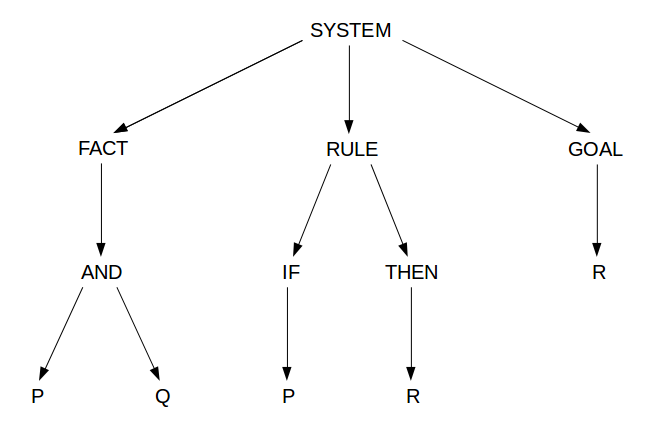
\includegraphics[width=12cm, height=8cm]{figures/systree.png}
\caption[Tree representation of a system]{\label{figtree}Tree representation of a system where there is a fact \(P \land Q\) and a rule \(P \rightarrow R\), with a goal of $R$.}\end{center}\end{figure}

In the example used in Figure \ref{figtree}, each component of the system is separate, but still linked, to every other component. It is then a simple matter to search the tree for desired nodes, such as the child of the goal node, $R$, as each node can be taken individually and compared, in context, to see if it yields a match. 

\subsection{Implementation}
With these considerations in mind, a grammar was created to outline the specification of rules for a system. These rules extend first order logic with notions of obligation, prohibition and permission. The grammar consists of parser rules and lexer rules. 

The lexer rules include `OB', `PRO' and `PER' to represent obligation, prohibition and permission, as well as lexer rules for common first order logic operators including `not', `and', `or', `if' and `then'. These are represented as words rather than symbols, particularly `then' rather than the implication symbol `$\rightarrow$' because it makes the code more readable for the person specifying the rules of the system. Terms are used so that atoms or propositions of the system can be referred to using symbols rather than their textual content, in order to maintain consistency and simplify the input. Assigning of atoms to symbols to create a term is done with `:', as this is more intuitive in context than a more traditional `='. 

The parser rules start with the program, which is made up of declarations, which are divided into declarations of terms, in the form of `C: some statement', declarations of facts, declarations of rules and declarations of goals. Facts, rules and goals are compound expressions. Expressions are divided into simple terms, prefix expressions, infix expressions and if...then expressions. Simple terms are denoted by a single identifier, and pick out some term in the data set. Prefix expressions have a prefix operator before some kind of expression; prefix operators are `not, `OB', `PRO' and `PER'. Infix expressions have an infix operator between two expressions; infix operators are `and' and `or'. If...then expressions have an expression enclosed by the IF operator and the THEN operator, with a second expression following the THEN operator. 

ANTLR is used to generate a lexer and parser for the grammar. Once a system has been specified in a file which respects the rules of the grammar, an ANTLR tree is generated. The tree divides the various components of the file into nodes in order to represent the input file in a structured manner. Some parser rules have rewrite rules to denote their representation in this tree. For example, the rewrite rule for a goal declaration is `DECL goal', which indicates that the parent node for this declaration in the tree will be `DECL', with the content of the goal as the child of that node. Where there are more than two elements of the system in the rewrite rule, the first represents the parent node, and every element following represent children nodes. 

The generated ANTLR tree will be used for the next stage of the tool, the prover. 

\subsection{Limitations}
One limitation of the formalised specification is the reliance on brackets to disambiguate expressions, particularly to make clear which expression a term belongs to. Brackets enclose prefix expressions, infix expressions and if...then expressions, but not identifiers, which is fairly intuitive. Identifiers are single terms, and do not need to be disambiguated. However, expressions are complex, and involve at least one operator and at least one identifier, so it is vital that it is clarified where the expression ends. Nevertheless, this could lead to confusion, and requires some documentation to make it obvious in which cases brackets are required by the grammar in order for the specification to be correctly parsed into an ANTLR tree. 

An additional limitation of the specification is that it does not include biconditionals in its parser 
rules. Due to considerations of time, this was removed, as implementing expressions containing 
biconditionals yields difficulties for the proof strategy. The biconditional operator $\iff$ is an 
infix 
operator, and an expression containing a biconditional would be treated as an infix expression. However, it does not seem entirely appropriate to consider biconditional along with the other infix operators, 'and' and 'or'. It has more in common with an if...then expression, which is an implication rule, than a conjunction or a disjunction. Consequently, there would be difficulties evaluating infix expressions in order to determine whether it should be treated as an implication rule or as a conjunction or disjunction. 

However, while this limitation is a concern, the specification has been designed in such a way that it is easily extendable. It would be fairly simple to add this rule to the specification once it had been correctly implemented in Deo's prover stage. 

\section{Proof Strategy}

\subsection{Design}
The prover will use a brute force proof strategy to prove, given a set of facts and a goal, that these facts cohere with the defined set of rules to produce the desired goal, or not, as the case may be. It will walk each node of the tree, and recursively check whether it and its children nodes match the facts required to yield new facts. The prover should make use of rules of inference and rules of replacement as part of its strategy \cite{infrules}. 

Critical rules to implement are modus ponens and modus tollens. Modus ponens affirms the antecedent of an argument; true premises guarantee true conclusions, so affirming the antecedent proves that the consequent is true. Modus tollens denies the consequent of an argument; false conclusions cannot follow true premises, so denying the consequent proves that the antecedent is false. These are foundational logical principles, and any prover would be sorely lacking without an implementation of them. They are crucial for the extraction of new facts; if some fact holds for one side of the rule, the truth of the other side can be asserted, and so it can be added to the fact set. 

A crucial rule to implement in terms of deontic logic is the rule of O-necessitation. If $A$ has been proven, OB ($A$) can be assumed, as no further step is required to prove OB ($A$). Furthermore, since $A$ entails OB ($A$), if OB($A$) has been proven then A can be assumed. This is a straightforward application of the modus ponens rule. In a similar fashion, if $\neg A$ has been proven, PRO ($A$) can be assumed, as prohibitions can also be formulated as OB ($\neg A$). There is nothing similar with permissions, as they can be formulated as $\neg$ OB ($A$) $\land$ $\neg$ OB($\neg A$), so these can be discarded in the pursuit of further facts. 

\subsection{Implementation}
The prover first scans the generated ANTLR tree to yield the terms, facts, rules and goals specified by the system under review. The terms are stored in a dictionary, with the identifiers of the terms stored as keys and the content of the terms stored as values, so that the identifiers, used in the facts, rules and goals, can be later substituted for their actual content. The facts, rules and goals are each stored in separate lists, with each list storing the parent of each relevant node of the tree. 

The prover implements various rules of inference and replacement, including modus ponens and modus tollens, as well as the rule of O-necessitation. For every rule in its data set, it checks every currently existing fact in its data set using the rules of inference and replacement in order to determine whether it can yield any more facts, in the hope of proving, or disproving, each goal in its data set. 

This process continues while each desired goal is not yet in the fact set, and while progress in the process has been made. The process terminates when progress has not been made, which is to say that the prover has not been able to yield any new facts from the rules. 

Once the process has terminated, the program returns to standard output the success of the prover. This output contains first an assertion as to whether the goals of the specified system have been made, which is to say whether the desired goals are validated by the specified rules of the system and the relevant specified facts about the world. If the assertion is true, that the case is successful in meeting its goals, then the output also contains a list of the steps required to prove that this is the case. These steps include the rule of inference or replacement that was used to generate a new fact and the original fact, specified in terms of its content rather than an identifier, that was part of generating this new fact. 

\subsection{Limitations}
Any brute force prover will suffer from inefficiency. For each fact, many of the rules are run through unnecessarily. A more intelligent approach would analyse the fact set and the rules in order to determine which rules are beneficial to run for a given fact in order to achieve the desired goal. 

The prover only returns steps that were successful in yielding a new fact for the fact set. While this makes it clearer what rules have actually been employed in the process, it may be beneficial to see which rules are unsuccessful in yielding new facts, particularly if it was expected that they would, in fact, be successful. 

Additionally, it only returns a general statement of success or failure for the entire set of goals. It would be beneficial for it return the steps followed and the status of proof for each goal, so that it was clear which goals were successfully and unsuccessfully met by the systsem. This would be particularly useful with a large set of goals, where it may be important to understand which particular goals cause the process to fail. Within the context of codes of applications, the goal is usually only the granting of acceptance by the governing body, but if there were other goals, it would be interesting to be made aware of what specifically needs to be addressed in order to achieve success in the future. 

Furthermore, the prover is not able to return as output to the user the terms, facts, rules or goals of the specified system once these have been extracted from the tree. These would be beneficial to have the option of viewing, so that the user would not have to return to the semi-structured input file in order to find this information. Additionally beneficial would be the option to enter a fact and have returned everything that is entailed by that fact, particularly any related obligations, prohibitions or permissions. 

The prover is also unable to add or remove terms, facts, rules or goals once these have been extracted. Having the option to do so available would enable the user to amend their specified system without having to quit the program, amend the input file and run the program again. 

However, while there is clear benefit to implementing both these functions, doing so does not fit with the main concerns of the prover, which are to carry out a brute force strategy on a fact and rule set. Instead, it would be beneficial to couple Deo with another tool whose purpose was to carry out the aforementioned additionally useful functionality. 

\chapter{Evaluation}

\section{Motivation, Expected Results and Methodology}
The purpose of this evaluation is to assess the performance of the prover, by comparing the results it produces against the actual results obtained by each case study examined. Successful results in this area will suggest proper functionality of the prover, which will suggest that it has been implemented well. 

The evaluation is carried out using four case studies. Case studies A, B and C are adapted from ethics applications of research proposals submitted to the University of Glasgow. These applications were obtained under a Freedom of Information request, which sought the documents of the first fifty applications approved within the College of Science and Engineering in the year 2012. The applications consist of an application form, a participant information sheet and a consent form. The applications do not contain experimental materials, results or data. Not only is this sensitive information, it is not necessary for the specification of each case study, and so does not fall under the purview of a reasonable request. 

The final case study, D, is not adapted from this set of applications. Rather, it is a fictitious case specifically designed to produce certain output from the prover. As all of the applications obtained from the University of Glasgow were from projects that were approved by the committee, case studies A, B and C are expected to yield success when tested against the prover, while case study D is designed to yield failure. 

Another aspect of this evaluation is the examination of the steps followed by the prover in its attempt to attain the goals of each case study. This examination cannot be validated by actual, external results, since all that is known of the case studies is that they were successful in achieving approval from the committee, and not why. However, the examination can suggest further points of consideration regarding the performance of the prover, in more depth than a simple validation of success. Potential points of consideration include the efficiency of the proof strategy. 

\section{Case Study A: Impacts of Climate Change, Variability and Agriculture Adaptation}

This first case study is an ethics proposal submitted by a postgraduate student from the School of Geographical and Earth Sciences [Appendix \ref{casestudyA}]. The proposed research project involves investigating rural communities and climate change, and the impacts it has on agriculture. This investigation involves carrying out interviews, questionnaires, structured observations, guided transect walk observations and oral histories. The subjects of the investigation are highland and lowland plains farmers, who are sent questionnaires and then randomly sampled for further participation. There is no anticipated effect on the physical wellbeing of the participants, but due to the sensitive nature of the investigation, participants may show signs of distress during interviews. In the case of such, the interview is immediately stopped. 

In addition to this, all the usual guidelines for the use of human participants in research projects are followed. The nature of the research is explained to the participants, whose informed, voluntary consent is sought, and whose anonymity is protected if desired. Consent to participate in the research project may be withdrawn at any time, and a participant's consent does not entail a requirement to answer every question that is asked of them, if the participant does not wish to answer a question. Every effort is made to make the participants comfortable, including limiting noise and external disturbance. Additionally, the pool of participants does not contain members of vulnerable groups. 

I specified this study as follows: 
\begin{verbatim}
A: "study has physical effects on participants"
B: "participant shows signs of distress during their interview"
C: "stop interviewing participant"
D: "study involves human participants"
E: "study involves members of vulnerable groups"
F: "explain the full nature of the research to the participants"
G: "offer anonymity to the participants"
H: "participants participate"
I: "participants disengage from the study at any point"
J: "participants respond or not respond to any question asked during 
    the interview"
K: "researcher will respect all wishes expressed by all participants"
L: "interviews will be conducted in areas where participants feel 
    comfortable"
M: "study is approved"
fact: (not A)
rule: (if B then C)
fact: D
fact: (not E)
fact: F
fact: G
fact: H
fact: I
fact: J 
fact: K
fact: L
rule: (if D then (((((((OB F) and (OB G)) and (PER H)) and (PER I)) and 
       (PER J)) and (OB K)) and (OB L)))
rule: (if (not D) then M)
rule: (if (D and (F and (G and (K and L))))) then M)
goal: M
\end{verbatim}

The results of this case study are as follows: 
\begin{verbatim}
Step 1: 
INITIAL: D
FINAL: (((((((OB F) and (OB G)) and (PER H)) and (PER I)) and (PER J)) and
        (OB K)) and (OB L))
TRANSFORM: (if D then (((((((OB F) and (OB G)) and (PER H)) and (PER I)) 
            and (PER J)) and (OB K)) and (OB L)))
RULE: modus ponens

Step 2: 
INITIAL: (D and (F and (G and (K and L))))
FINAL: M
TRANSFORM: (if (D and (F and (G and (K and L)))) then M)
RULE: modus ponens


STATUS: success
\end{verbatim}

As expected, this application was successful in meeting the requirements to proceed with the desired research. Its success is derived from the existence of required facts in the fact set, namely D, F, G, K and L. Their conjunction as the antecedent of the case study rule (if (D and (F and (G and (K and L))))) then M) entails the consequent, M, which is the goal of this case study. Using the rule of modus ponens, where affirming the antecedent affirms the consequent, M was extracted as a new fact. 

This is a direct application of the fact set to a rule, and takes only one step. However, the prover took two steps to establish the success of the case study. The first step applied the rule of modus ponens to the case study rule (if D then (((((((OB F) and (OB G)) and (PER H)) and (PER I)) and (PER J)) and (OB K)) and (OB L))), and used the fact D to extract as a new fact (((((((OB F) and (OB G)) and (PER H)) and (PER I)) and (PER J)) and (OB K)) and (OB L))). This step, however, yielded no new useful facts for the fact set. Permissions can be discarded as they are neither true nor false, and the facts tied to the obligations which are validated as true already exist in the fact set. 

\section{Case Study B: Digigraff}
The second case study is an ethics proposal submitted by a student in the School of Computing Science [Appendix \ref{casestudyB}]. The proposed research project aims to investigate the role of location in the creation of social media content, and to encourage users to be more thoughtful about location in their use of social media. These aims are met through an evaluation of DigiGraff, which allows users to create digital annotations that can be projected onto physical surfaces and then stored, along with the location of the user in their physical environment. The project is carried out remotely in three phases, with experimenter contact only in the first and third phase. The first phase involves the provision of information about the project to participants and the gathering of consent. The second phase involves actual use of DigiGraff for the period of a week. The third phase involves interviewing the participants about their experience using DigiGraff. 

The student anticipates minimal physical effect on the participants of the research project. Any effects concern the comfort, safety and privacy of the participants, all of which they are made aware of the protection of before the project begins. All of the usual ethical guidelines are followed, and no members of vulnerable groups will be recruited for the project. 

I specified this case study as follows: 
\begin{verbatim}
P: "involve participation of other people"
Q: "involve data relating to other people"
R: "complete ethics checklist form"
S: "apply for ethical approval"
T: "comply with points on ethics checklist form"
U: "use introduction and debriefing scripts"
V: "include introduction and debriefing scripts with signed ethics checklist 
    form as part of report"
W: "study approved"
rule: (if (P or Q) then R)
rule: (if (((P or Q) and R) and (not T)) then (OB ((S and U) and V)))
rule: (if (T or (S and (U and V)) then W)
fact: P
fact: Q
fact: (not T)
goal: W
\end{verbatim}

The results of this case study are as follows: 
\begin{verbatim}
Step 1: 
INITIAL: (P or Q)
FINAL: R
TRANSFORM: (if (P or Q) then R)
RULE: modus ponens

Step 2: 
INITIAL: (((P or Q) and R) and (not T))
FINAL: (OB ((S and U) and V))
TRANSFORM: (if (((P or Q) and R) and (not T)) then (OB ((S and U) and V)))
RULE: modus ponens

Step 3: 
INITIAL: (OB ((S and U) and V))
FINAL: ((S and U) and V)
TRANSFORM: (OB ((S and U) and V))
RULE: O necessity

Step 4: 
INITIAL: (S and U)
FINAL: S
TRANSFORM: (S and U)
RULE: decompose conjunction

Step 5: 
INITIAL: (S and U)
FINAL: U
TRANSFORM: (S and U)
RULE: decompose conjunction

Step 6: 
INITIAL: ((S and U) and V)
FINAL: V
TRANSFORM: ((S and U) and V)
RULE: decompose conjunction

Step 7: 
INITIAL: (T or (S and (U and V)))
FINAL: W
TRANSFORM: (if (T or (S and (U and V))) then W)
RULE: modus ponens


STATUS: success

\end{verbatim}
As expected, this application was successful in meeting the requirements to proceed with the desired research. There are several steps necessary to reach this proof. Firstly, the existence of the facts P and Q is used to yield the fact R from the case study rule if (P or Q). Secondly, the existence of the facts P, Q and not T, as well as the newly extracted rule, R, is used to yield the fact (OB ((S and U) and V)) from the case study rule (if (((P or Q) and R) and (not T)) then (OB ((S and U) and V). Thirdly, the rule of O-necessitation is used to extract the facts S, U and V, decomposed from their original conjunction. Finally, these extracted facts are used to yield the fact W, which is the goal of this case study, from the case study rule (if (T or (S and (U and V)) then W). 

Unlike with Case Study A, the prover followed exactly this number of steps in order to achieve the case study's stated goal. All the case study rules create new facts for the fact set. There are no irrelevant case study rules; every rule advances the prover further along its route to a proof. The proof strategy works optimally with this kind of case study, but it is hardly a typical or even likely case. Particularly with ethics applications, it may not be clear what information is relevant, or what rules are likely to lead to the creation of new facts when the fact set is applied. Regardless, it is the responsibility of the prover to determine which facts and rules are relevant to the pursuit of the goals, not the specifier of the facts, rules and goals. 

\section{Case Study C: High Places, Unique Spaces}
The third case study is an ethics proposal submitted by a student in the School of Geographical and Earth Sciences [Appendix \ref{casestudyC}]. The proposed research project aims to investigate relationships created while trekking and mountaineering in the Himalayas, and involves engaging with the international trekking and mountaineering community and the differences between these groups. The project involves conducting semi-structured interviews with the Himalayan mountaineering community, where key information about the participants and physical reactions will be recorded as well as audio of the interviews. It also involves carrying out ethnographic research, which entails the student participation themselves in mountaineering activities, and conducting discourse analysis of policy documents in the public domain. 

The student does not anticipate any negative effects on the participants, though the project is quite intensive and may trigger emotional responses in the participants, who will be made aware that they can withdraw their consent to participate or simply choose not to answer the question. Efforts will be made to minimise any disruption to the participants' lives and continual operation of their occupations. A further source of ethical considerations is the cultural context and inherent power relations between researcher and participant, due to the Western/Eastern divide. Efforts will be made to adhere to cultural norms. Finally, no members of vulnerable groups will be participants in the study. Some participants may be illiterate, and in this case, an oral explanation of the terms of participation will be delivered and verbal consent will be sought. 

I specified this case study as follows: 
\begin{verbatim}
A: "cultural power relations exist"
B: "be culturally sensitive"
C: "observe cultural norms"
D: "language and culture barriers exist"
E: "ask for clarification"
F: "conduct interviews a the end of each stay"
G: "photography and video is taken"
H: "permission of individuals involved is sought"
I: "document exists in the public domain"
J: "document is used in research"
K: "participant participates"
L: "participant withdraws at any time"
M: "participants are anonymised"
N: "paricipants answer interview questions"
O: "participants are members of vulnerable groups"
P: "participants are illiterate"
Q: "verbal consent sought"
R: "study is approved"
fact: A
fact: D
fact: G
fact: I
fact: K
fact: (if A then D)
fact: P
fact: (not O)
rule: (if A then (OB (B and C)))
rule: (if D then (OB (E and F)))
rule: (if G then (OB H))
rule: (if I then (PER J))
rule: (if K then (PER ((L and M) and N)))
rule: (if P then Q)
rule: (if (((((((((A and B) and C) and D) and E) and F) and G) and H) and 
       P) and Q) then R)
goal: R
\end{verbatim}

The results of this case study are as follows: 
\begin{verbatim}
Step 1: 
INITIAL: A
FINAL: (OB (B and C))
TRANSFORM: (if A then (OB (B and C)))
RULE: modus ponens

Step 2: 
INITIAL: D
FINAL: (OB (E and F))
TRANSFORM: (if D then (OB (E and F)))
RULE: modus ponens

Step 3: 
INITIAL: G
FINAL: (OB H)
TRANSFORM: (if G then (OB H))
RULE: modus ponens

Step 4: 
INITIAL: I
FINAL: (PER J)
TRANSFORM: (if I then (PER J))
RULE: modus ponens

Step 5: 
INITIAL: K
FINAL: (PER ((L and M) and N))
TRANSFORM: (if K then (PER ((L and M) and N)))
RULE: modus ponens

Step 6: 
INITIAL: P
FINAL: Q
TRANSFORM: (if P then Q)
RULE: modus ponens

Step 7: 
INITIAL: (OB (B and C))
FINAL: (B and C)
TRANSFORM: (OB (B and C))
RULE: O necessity

Step 8: 
INITIAL: (OB (E and F))
FINAL: (E and F)
TRANSFORM: (OB (E and F))
RULE: O necessity

Step 9: 
INITIAL: (OB H)
FINAL: H
TRANSFORM: (OB H)
RULE: O necessity

Step 10: 
INITIAL: (B and C)
FINAL: B
TRANSFORM: (B and C)
RULE: decompose conjunction

Step 11: 
INITIAL: (B and C)
FINAL: C
TRANSFORM: (B and C)
RULE: decompose conjunction

Step 12: 
INITIAL: (E and F)
FINAL: E
TRANSFORM: (E and F)
RULE: decompose conjunction

Step 13: 
INITIAL: (E and F)
FINAL: F
TRANSFORM: (E and F)
RULE: decompose conjunction

Step 14: 
INITIAL: (((((((((A and B) and C) and D) and E) and F) and G) and H) and P) and Q)
FINAL: R
TRANSFORM: (if (((((((((A and B) and C) and D) and E) and F) and G) and H) and P) and Q) then R)
RULE: modus ponens


STATUS: success
\end{verbatim}
As expected, this application was successful in meeting the requirements to proceed with the proposed research. There are several steps necessary to reach this goal. Firstly, the existence of the fact A is used to yield the fact OB(B and C) from the case study rule (if A then (OB (B and C))). After applying the O-necessitation rule and decomposing the conjunction, the facts B and C are extracted. Simarly, D is used to yield the fact OB(E and F) from the case study rule (if D then (OB (E and F))), and then the facts E and F are extracted. G is used to yield the fact OB H from the case study rule (if G then (OB H)), and then the fact H is extracted. Finally, P is used to yield Q from the case study rule (if P then Q). All the facts needed to affirm the antecedent of the case study rule (if (((((((((A and B) and C) and D) and E) and F) and G) and H) and P) and Q) then R) now exist in the fact set, so the goal of the case study, R, can be extracted. 

As with Case Study A, the prover took more steps than were strictly required. This is a bit more complicated as an example, and it is even less obvious which rules are relevant to the prover's goals, at least without manually executing the process. However, it is interesting to note that, again, it is the rules involving permissions, which yield no new facts for the fact set when there are no permissions involved in the route to the goal, that are uselessly applied. 

\section{Case Study D: Lack of Participant Consent}
The final case study is an ethics application for a fictional research project. This case study is designed to fail, so it includes human participants and also a prohibition on seeking consent of participants, where the rules of the code of ethics are that if there are human participants in a study, the researcher must seek the consent of the participants of the study, and if consent is not sought, then approval of the study is not granted. 

I specified this case study as follows: 
\begin{verbatim}
P: "human participants in study" 
Q: "seek consent of participants"
R: "study approved"
rule: (if P then Q)
rule: (if (not Q) then (not R))
fact: (PRO Q)
goal: R
\end{verbatim}

The results of this case study are as follows: 
\begin{verbatim}
Step 1: 
INITIAL: (PRO Q)
FINAL: (not Q)
TRANSFORM: (PRO Q)
RULE: O necessity

Step 2: 
INITIAL: P
FINAL: (not P)
TRANSFORM: (if P then Q)
RULE: modus tollens

Step 3: 
INITIAL: (not Q)
FINAL: (not R)
TRANSFORM: (if (not Q) then (not R))
RULE: modus ponens


STATUS: failure
\end{verbatim}
The result of failure is as expected; the case study was designed so that, were it real, it should have been approved by the committee. The proof strategy is as follows: derive the fact not Q from the fact PRO Q using the O-necessitation rule, derive the fact not R from the case study rule (if (not Q) then (not R)) using the fact not Q, then stop checking the rules as no new facts have been created. Since, at this point, the goal R does not exist in the fact set, the prover returns failure as the status of the case study. 

However, more important for the disproof of the goal than there being no new facts able to be generated is that the negation of the goal, not R, has been proved, rendering a proof of R either impossible or completely incoherent. The prover is unable to return this as a result; it can only fail to provide a proof for the goal, not disprove it. 

\chapter{Conclusions and Future Work}

\section{Conclusions}
Through continual assessment of the tool itself and the formal evaluation of case studies, it is clear that Deo has several limitations. It is evident from the case studies that sometimes many more steps are carried out by the prover than are strictly necessary in an attempt derive a proof of the goal. This redundancy is characteristic of brute force proof strategies, where rules are exhaustively applied in search of new facts, and could be addressed by a more intelligent analysis of the fact set before the application of rules. 

A further limitation of the prover is that it only returns a general statement of success or failure for the entire set of goals. The case studies examined here have only had one goal, so this was not an issue, but with a large set of goals, it would be benficial to return the steps followed and the status of proof for each goal. This would make it clearer which goals are responsible for the failure of the proof, and what action is required to remedy this. 

Additional limitations regard extraneous functionality to the proof strategy, such as the ability to return the atoms of the specified system as output to the user, as well as the ability to to add or remove atoms of the system outside of the original input file. These functions would be useful to implement in a tool to be used in conjunction with Deo. 

With regards the lexical specification, the reliance on brackets to disambiguate expressions is regrettable. With complex expressions, it quickly becomes difficult to keep track of which brackets enclose which expression. Even with the inclusion of examples with Deo, it is not entirely clear how brackets are required for disambiguation. For example, a conjunction that comprises three single terms must currently be represented either as (P and (Q and R)) or as ((P and Q) and R), since the two statements are equivalent. Much more intuitive would be to allow for this conjunction to be represented as (P and Q and R), but this is not possible within the current structure of the grammar. 

Despite these limitations, the project has met its stated objectives. It comprises a formalised specification of deontic logic and a deontic theorem prover, which works as expected with the test cases and provides thoughtful results for evaluation. With some extension, it will prove highly useful as a tool for using deontic logic to model systems, to set up deontic theorems to reason against, and to prove desired facts in a deontic manner. 

Overall, I am satisfied with Deo and the results it has yielded. It has been a rewarding and enjoyable experience to work on this project, and I have identified several areas for potential development and improvement. 

\section{Future Work}
One key strength of the prover is the more intuitive specification system, and the lack of esoteric symbolism, which makes Deo more accessible for the average user. However, it does not go far enough. There are some quirks to the specification that, while exemplified in the examples providied for the smooth running of the prover, are not at all immediately obvious. This could be avoided with a more intuitive interface, one which does not rely on human input to specify a system in the deontic grammar. 

One way of doing this would be to provide an additional graphical interface which allowed the user to enter the facts, rules and goals of a system in some kind of structured form, which was then processed to create the kind of file currently required of the user to produce by themselves. This would greatly reduce the number of errors faced by the user when specifying the system, simply because they have not understood the exact specification of the deontic grammar. It would also reduce the amount of time and effort required to use Deo, a key concern for its usability and potential benefit. 

When considering ways to supplement Deo's usability, the work done in automatic parsing of text has much to offer. Its functionality would be greatly improved if extended in conjunction with a tool which could scan documents, such as codes of ethics and completed ethics applications for projects, for key terms and information, in order to automatically generate a set of facts, rules and goals for a system.  

Equally, Deo has much to offer other areas of work. Its obvious uses are within any context that is concerned with ethics, and it would be beneficial to extend its application to more complex case studies, such as the British Psychological Society code of ethics \cite{bps_2016}. The document is very long, with lots of complex rules and guidelines. It would be challenging to formalise, but an evaluation with a case study of its complexity could yield interesting and perhaps unexpected results. As the rules get more numerous and more complicated, the relations between the fact set and the rule set may be manipulated in ways that were not initially intended during Deo's design and implementation. 

Additionally, the focus could be extended outside of the scope of ethics. Responsibility modelling is one such area where Deo could be very useful. Formalising responsibilities as obligations and prohibitions is already possible; this aspect of Deo's functionality could be coupled with a wider responsibility modelling framework in order to supplement the framework with deontic concepts. 

%%%%%%%%%%%%%%%%
%              %
%  APPENDICES  %
%              %
%%%%%%%%%%%%%%%%
\begin{appendices}
\chapter{Running the Programs}
README.txt contains instructions as to how to run the code. On a Linux machine, these are as follows. 

To install dependencies: 
\begin{verbatim}
pip install http://www.antlr3.org/download/Python/antlr_python_runtime-3.1.2.tar.gz
\end{verbatim}
To recompile the lexer and parser for the grammar: 
\begin{verbatim}
wget http://www.antlr3.org/download/antlr-3.1.2.jar
java -classpath "antlr-3.1.2.jar" org.antlr.Tool Deo.g
\end{verbatim}
To run the main component of the program (prover.py): 
\begin{verbatim}
python prover.py
\end{verbatim}

On a Windows machine, the commands are as follows. 

To install dependencies: 
\begin{verbatim}
curl https://bootstrap.pypa.io/ez_setup.py | python
curl https://bootstrap.pypa.io/get-pip.py | python
pip install http://www.antlr3.org/download/Python/antlr_python_runtime-3.1.2.tar.gz
\end{verbatim}

To recompile the lexer and parser for the grammar: 
\begin{verbatim}
curl http://www.antlr3.org/download/antlr-3.1.2.jar
java -classpath "antlr-3.1.2.jar" org.antlr.Tool Deo.g
\end{verbatim}

To run the main component of the program (prover.py): 
\begin{verbatim}
	python prover.py
\end{verbatim}

An example of running the prover from the command line is as follows:
\begin{verbatim}
pip install http://www.antlr3.org/download/Python/antlr_python_runtime-3.1.2.tar.gz
python prover.py
path to input file:
Tests/Unit_Tests/modusPonens-pass.deo
TREE: 
 === DECL ===
        === TERM ===
                === P ===
                === "it's sunny in Glasgow" ===
 === DECL ===
        === TERM ===
                === Q ===
                === "CS students work outside" ===
 === DECL ===
        === fact ===
                === P ===
 === DECL ===
        === rule ===
                === IFTHEN ===
                        === P ===
                        === Q ===
 === DECL ===
        === goal ===
                === Q ===

Step 1: 
INITIAL: P
FINAL: Q
TRANSFORM: (if P then Q)
RULE: modus ponens

STATUS: success
\end{verbatim}

\chapter{Case Studies}
\section{Case Study A}
\label{casestudyA}
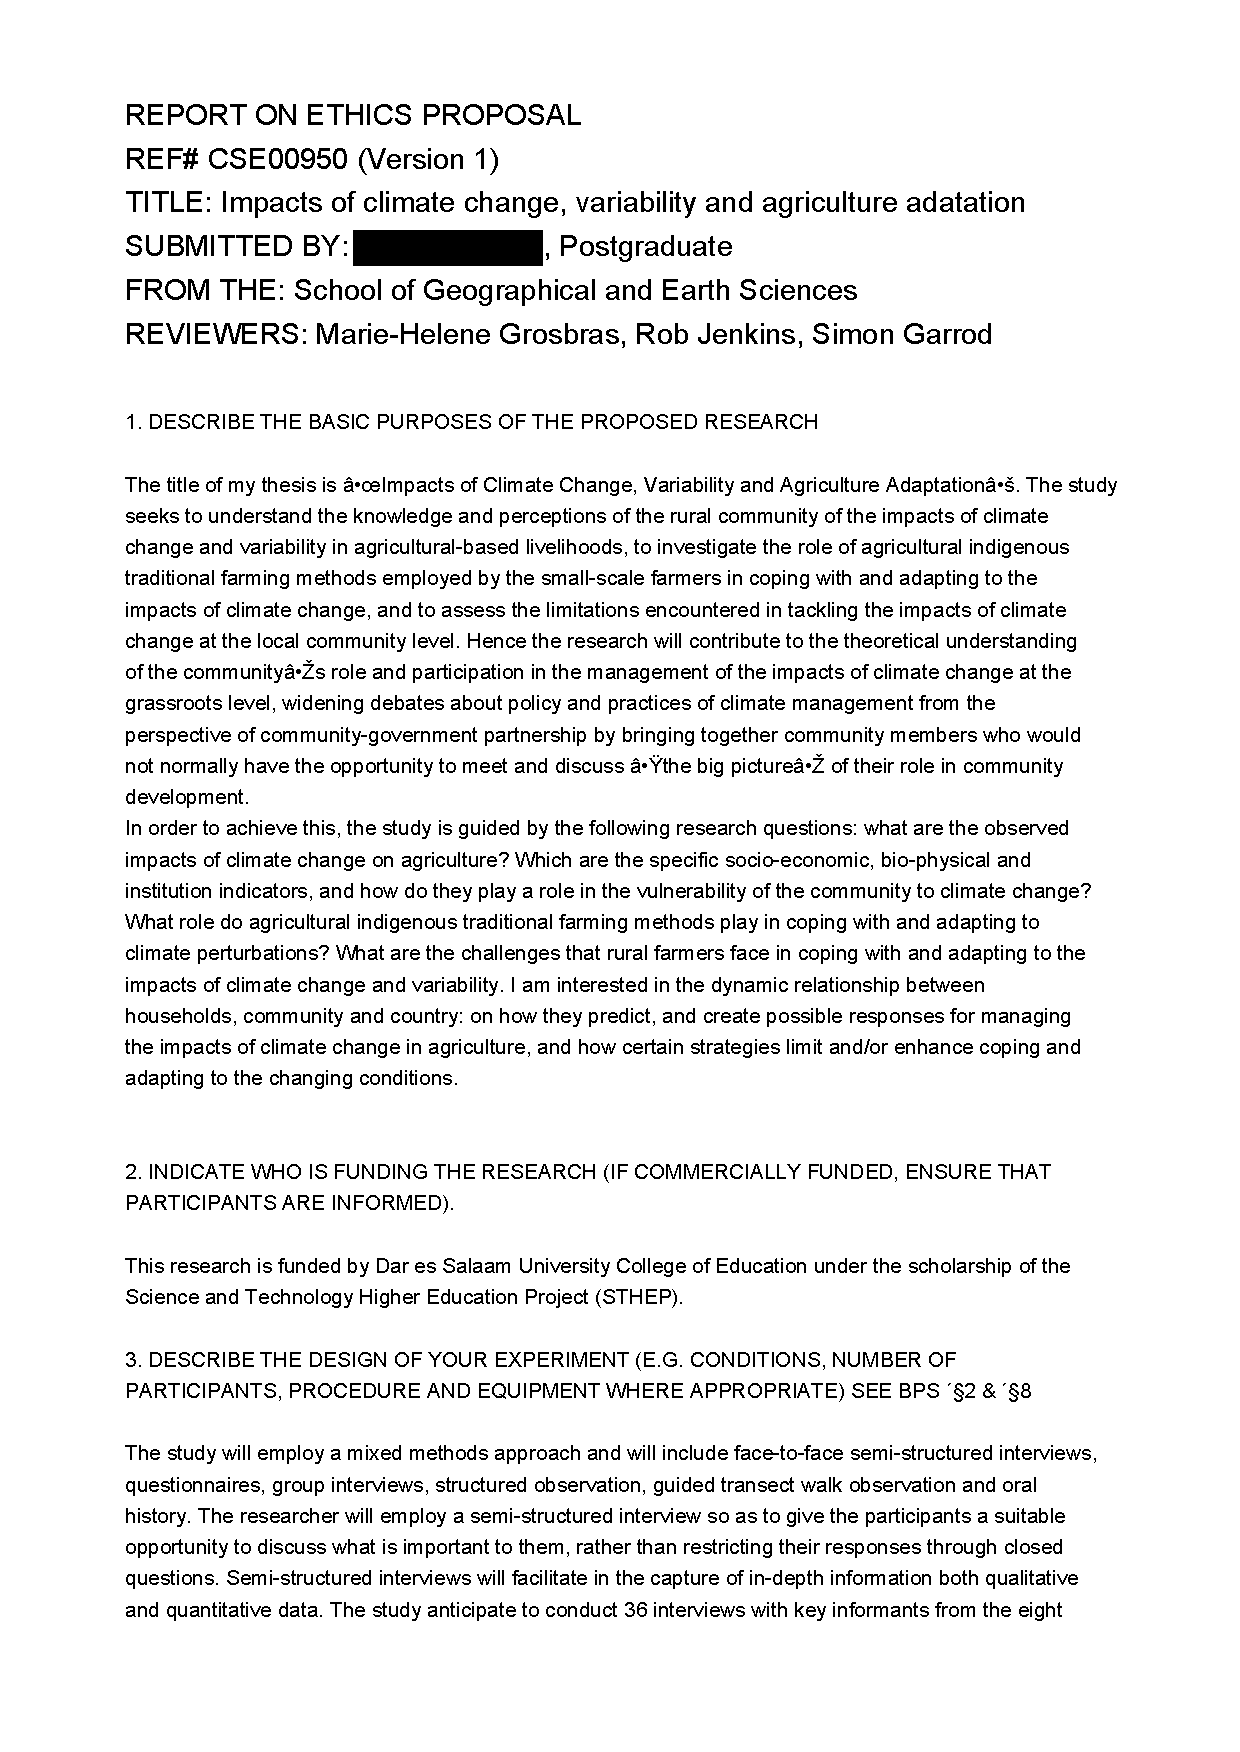
\includepdf[pages={1-8}]{ethicsapps/Appendix_A.pdf}
\section{Case Study B}
\label{casestudyB}
\includepdf[pages={50-55}]{ethicsapps/Appendix_B.pdf}
\section{Case Study C}
\label{casestudyC}
\includepdf[pages={34-41}]{ethicsapps/Appendix_E.pdf}

\end{appendices}

%%%%%%%%%%%%%%%%%%%%
%   BIBLIOGRAPHY   %
%%%%%%%%%%%%%%%%%%%%

\bibliographystyle{IEEEtran}
\bibliography{IEEEabrv,bib}

\end{document}
